%\documentclass[10pt,aspectratio=43,t,l]{beamer}
\documentclass[10pt,aspectratio=169,t,l,fleqn,mathsanserif,sanserif]{beamer}
%\documentclass[10pt]{beamer}

%\setbeamertemplate{footline}[page number]{}

\usepackage{framed}
\usepackage{tcolorbox}
\colorlet{shadecolor}{blue!15}
\usepackage{color,amsmath,xmpmulti,textpos,comment,eurosym,bm,amsthm,tabularx,cancel}
\usepackage{epsfig}
\usepackage{nicefrac}
\usepackage{listings}
%\usepackage{enumitem}
\usepackage{graphicx}    
\usepackage{graphics}
\usepackage{epstopdf}
\usepackage[normalem]{ulem}
\usepackage{float}
%\usepackage[cmbold]{mathtime}
%\usepackage{mt11p}
\usepackage{placeins}
\usepackage{amsmath}
\usepackage{pifont}
\usepackage{color}
\usepackage{amssymb}
\usepackage{mathtools}
\usepackage{subfigure}
\usepackage{multirow}
\usepackage{epsfig}
\usepackage{listings}
%\usepackage{enumitem}
\usepackage{rotating,tabularx}
%\usepackage[graphicx]{realboxes}
\usepackage{graphicx}
\usepackage{graphics}
\usepackage{epstopdf}
\usepackage{longtable}
%\usepackage[pdftex]{hyperref}
\usepackage{breakurl}
\usepackage{epigraph}
\usepackage{xspace}
\usepackage{amsfonts}
\usepackage{eurosym}
\usepackage{ulem}
\usepackage{footmisc}
\usepackage{comment}
\usepackage{setspace}
\usepackage{geometry}
\usepackage{caption}
\usepackage{pdflscape}
\usepackage{array}
\usepackage[round]{natbib}
\usepackage{booktabs}
\usepackage{dcolumn}
\usepackage{mathrsfs}
\usepackage{tikz}
\usetikzlibrary{decorations.pathreplacing}
\usepackage{sansmathaccent}
\pdfmapfile{+sansmathaccent.map}
\usetikzlibrary{shapes.geometric, arrows,chains}
\tikzset{
  startstop/.style={
    rectangle, 
    rounded corners,
    minimum width=3cm, 
    minimum height=1cm,
    align=center, 
    draw=black, 
    fill=red!30
    },
  startsleft/.style={
    rectangle, 
    rounded corners,
    minimum width=3cm, 
    minimum height=1cm,
    align=left, 
    draw=black, 
    fill=red!30
    },
  startsright/.style={
    rectangle, 
    rounded corners,
    minimum width=3cm, 
    minimum height=1cm,
    align=right, 
    draw=black, 
    fill=red!30
    },
  process/.style={
    rectangle, 
    minimum width=3cm, 
    minimum height=1cm, 
    align=center, 
    draw=black, 
    fill=blue!30
    },
  decision/.style={
    rectangle, 
    minimum width=3cm, 
    minimum height=1cm, align=center, 
    draw=black, 
    fill=green!30
    },
  arrow/.style={thick,->,>=stealth},
  dec/.style={
    ellipse, 
    align=center, 
    draw=black, 
    fill=green!30
    },
  font={\fontsize{9pt}{12}\selectfont}
}
%\renewcommand{\labelitemi}{$\blacktriangleright$}

\epstopdfsetup{outdir=./}

\newcolumntype{Y}{>{\centering\arraybackslash}X}
\def\Put(#1,#2)#3{\leavevmode\makebox(0,0){\put(#1,#2){#3}}}

\newcommand{\subhead}[1]{\mbox{}\newline\textbf{#1}\newline}
\newcommand{\ave}[1]{\left\langle #1 \right \rangle}
\newcommand{\eg}{{\it e.g.}}
\newcommand{\ie}{{\it i.e.}}
\newcommand{\cf}{{\it c.f.}}
\newcommand{\etc}{{\it etc.}}
\newcommand{\etal}{{\it et al.}}
%\newcommand{\btVFill}{\vskip0pt plus 1filll}

\newcommand{\del}{D}
\newcommand{\hor}{H}

\newcommand{\threepartdef}[6]
{
  \left\{
    \begin{array}{lll}
      #1 & \mbox{if } #2 \\
      #3 & \mbox{if } #4 \\
      #5 & \mbox{if } #6
    \end{array}
  \right.
}


\newcommand{\Ito}{It\^{o}}
\newcommand{\SP}{S{\&}P500}
\newcommand{\lopt}{\ell_{\text{opt}}}
\newcommand{\gest}{g_{\text{N,T}}}
\newcommand{\elabel}[1]{\label{eq:#1}}
\newcommand{\eref}[1]{Eq.~(\ref{eq:#1})}
\newcommand{\Eref}[1]{Equation~(\ref{eq:#1})}

\newcommand{\flabel}[1]{\label{fig:#1}}
\newcommand{\fref}[1]{Fig.~\ref{fig:#1}}
\newcommand{\Fref}[1]{Figure~\ref{fig:#1}}
\newcommand{\person}[1]{{#1}}
\newcommand{\ra}[1]{\renewcommand{\arraystretch}{#1}}
\newcommand{\vs}[1]{\vspace{.#1cm}}
\newcommand{\vf}{\vspace{.25cm}}
\newcommand{\vff}{\vspace{.6cm}}
\newcommand{\np}{\\ \vf}
\newcommand{\npp}{\\ \vff}
\newcommand{\be}{\begin{equation*}}
\newcommand{\ee}{\end{equation*}}
\newcommand{\bea}{\begin{eqnarray*}}
\newcommand{\eea}{\end{eqnarray*}}
\newcommand{\bc}{\begin{center}}
\newcommand{\ec}{\end{center}}
\newcommand{\bie}{\begin{enumerate}}
\newcommand{\eie}{\end{enumerate}}
\newcommand{\bi}{\begin{itemize}}
\newcommand{\ei}{\end{itemize}}
\newcommand{\toinf}{\rightarrow\infty}
\newcommand{\D}{{\Delta}}
\newcommand{\Dx}{{\Delta x}}
\newcommand{\Dy}{{\Delta y}}
\newcommand{\Du}{{\Delta u}}
\newcommand{\DW}{{\Delta W}}
\newcommand{\DU}{{\Delta U}}
\newcommand{\du}{{\delta u}}
\newcommand{\Dv}{{\Delta v}}
\newcommand{\dt}{{\delta t}}
\newcommand{\gens}{g_{\ave{\,}}}
\newcommand{\ft}[1]{\frametitle{#1}}
\newcommand{\bq}{\begin{quote}}
\newcommand{\eq}{\end{quote}}
\newcommand{\ww}[1]{\bq{\small\rm#1\\}\eq}
\newcommand{\E}{\mathrm{E}}
\newcommand{\Var}{\mathrm{Var}}
\newcommand{\Cov}{\mathrm{Cov}}
\newcommand{\sgn}{\mathrm{sgn}}
\newcommand{\prob}[1]{\mathcal{P}\left(#1\right)}
\newcommand{\lra}{\longrightarrow}
\newcommand{\eps}{\varepsilon}
\newcommand{\ga}{g_\text{ave}}
\newcommand{\gt}{g_\text{typ}}
\newcommand{\gbar}{\bar{g}}
\newcommand{\mbar}{\bar{m}}
\newcommand{\red}[1]{\textcolor{red}{#1}}
\newcommand{\xf}{{x_F}}
\newcommand{\xb}{{x_B}}
\newcommand{\muf}{{\mu_F}}
\newcommand{\mub}{{\mu_B}}
\newcommand{\sigf}{{\sigma_F}}
\newcommand{\sigb}{{\sigma_B}}
\newcommand{\gf}{{\gbar_F}}
\newcommand{\gb}{{\gbar_B}}
\newcommand{\pa}{\textit{pa}}
\newcommand{\taus}{{\tau_\text{s}}}
\newcommand{\Dt}{\Delta t}
\newcommand{\etau}{\tau^\text{eqm}}
\newcommand{\taue}{\tau^\text{EGBM}}
\newcommand{\wtau}{\widetilde{\tau}}
\newcommand{\xN}{\ave{x}_N}
\newcommand{\Sdata}{S^{\text{data}}}
\newcommand{\Smodel}{S^{\text{model}}}
\beamertemplatenavigationsymbolsempty

\newcommand{\tlabel}[1]{\label{tab:#1}}
\newcommand{\tref}[1]{Tab.~\ref{tab:#1}}
\newcommand{\Tref}[1]{Table~\ref{tab:#1}}

\newenvironment{myindentpar}[1]%
{\begin{list}{}%
    {\setlength{\leftmargin}{#1}}%
  \item[]%
}
{\end{list}}

%\usetheme[width=1.8cm,hideothersubsections]{Frankfurt}
\usetheme{Frankfurt}

\newcommand\BackgroundPicture[1]{
\setbeamertemplate{background}{
\parbox[c][\paperheight]{\paperwidth}{
\vfill \hfill
\includegraphics[width=1\paperwidth,height=1\paperheight]{#1}
\hfill \vfill
}}}


\definecolor{lmlblue}{RGB}{0,77,123}
\definecolor{deepblue}{RGB}{35,33,169}
\definecolor{lmllb}{RGB}{237,244,255}
\definecolor{lmlred}{RGB}{155,29,29}
\definecolor{lmlgrey}{RGB}{142,142,142}
\definecolor{lmlgrey2}{RGB}{82,82,82}
\definecolor{grey}{RGB}{210,210,210}
\xdefinecolor{lightblue}{rgb}{0,200,255}
\setbeamercolor{important}{bg=lightblue,fg=red}
\AtBeginEnvironment{definition}{%
  \setbeamercolor{block body}{fg=black,bg=white}
  \setbeamercolor{block title}{bg=lmllb,fg=black}
}

\AtBeginEnvironment{theorem}{%
  \setbeamercolor{block body}{fg=black,bg=white}
  \setbeamercolor{block title}{bg=lmllb,fg=black}
}

%\newcommand{\propnumber}{} % initialize
%\newtheorem*{prop}{Proposition \propnumber}
%\newenvironment{propc}[1]
%  {\renewcommand{\propnumber}{#1}%
%   \begin{shaded}\begin{prop}}
%  {\end{prop}\end{shaded}}
%\AtBeginEnvironment{propc}{%
%  \setbeamercolor{block body}{fg=black,bg=white}
%  \setbeamercolor{block title}{bg=lmllb,fg=black}
%}

\setbeamercolor{fine separation line}{fg=lmllb}

\setbeamercolor{item projected}{fg=white, bg=black}

\setbeamercolor{frametitle}{bg=lmllb, fg=black}
\setbeamertemplate{frametitle}[default][left,colsep=-4bp,rounded=false,shadow=false]

\setbeamercolor{structure}{bg=white, fg=black}
%structure changes color of title in sidebar.

%\setbeamertemplate{frametitle}[default][colsep=-4bp,rounded=false,shadow=false]
\setbeamercolor{section in head/foot}{fg=lmlgrey2, bg=lmllb}
\setbeamercolor{normal text}{fg=black}
\setbeamercolor{title}{bg=white,fg=deepblue}

\hypersetup{colorlinks,linkcolor=,urlcolor=deepblue}

\setbeamerfont{title in sidebar}{size=\fontsize{9}{9}\selectfont}
\setbeamerfont{section in sidebar}{size=\fontsize{7}{7}\selectfont}

% add frame numbers to navigation bar
% (for RSS 2015 conference)
\addtobeamertemplate{navigation symbols}{}{
    \usebeamerfont{footline}
    \usebeamercolor[fg]{footline}
    \hspace{1em}
    \scriptsize
%    \insertframenumber/\inserttotalframenumber
}
\setbeamertemplate{navigation symbols}{} %gets rid of navigation symbols
\setbeamercovered{transparent=20}
%\setbeamertemplate{footline}[frame number] % to show overlay page numbers type: page number
%\setbeamersize{text margin left=0.65cm, text margin right=0.65cm}
%\setbeamercolor{item}{fg=black!70!black} % red bullets
%\setbeamertemplate{itemize subitem}[triangle] % triangle sub-bullets
%\setbeamerfont{itemize/enumerate subbody}{size=\normalsize}


\title[\begin{flushleft} \color{white} {\tiny ???} \end{flushleft}]{\bf {Industrial Organization, Week 5 \\ 
Hotelling}}
\author[shortname]{ Dio Mavroyiannis \inst{\dag}}
\institute[\begin{flushleft} \color{white} {\large ???} \end{flushleft}]{Milestone Institute}
%\institute[shortinst]{\inst{*} London Mathematical Laboratory \and \inst{\dag} Universit\'{e} Paris-Dauphine \and \inst{\ddag} London Mathematical Laboratory and Santa Fe Institute}
\date{03 March 2021}

\AtBeginSection[]{
\frame{
\ft{Agenda}
\tableofcontents[currentsection,hideallsubsections]
}
}

\makeatletter
\setbeamertemplate{headline}{%
  \pgfuseshading{beamer@barshade}%
  \ifbeamer@sb@subsection%
    \vskip-9.75ex%
  \else%
    \vskip-7ex%
  \fi%
    \begin{beamercolorbox}[ht=3.5ex,dp=2.125ex]{section in head/foot}
     \insertsectionnavigationhorizontal{\textwidth}{}{}%
  \end{beamercolorbox}%
  \ifbeamer@sb@subsection%
    \begin{beamercolorbox}[ignorebg,ht=2.125ex,dp=1.125ex,%
      leftskip=.3cm,rightskip=.3cm plus1fil]{subsection in head/foot}
      \usebeamerfont{subsection in head/foot}\insertsubsectionhead
    \end{beamercolorbox}%
  \fi%
}%

\makeatother

\setbeamertemplate{mini frames}{}
\setbeamertemplate{itemize items}[triangle]

\begin{document}
\frame{\titlepage\insertlogo}

\section{Big picture}
%%%%%%%%%%%%%%%%%%%%%%%%%%%%%%%%%%%%%%%%%%%%%
\frame{\ft{Dynamic}
\setbeamertemplate{itemize items}[triangle]

\bi
\item Plan: We look at our third dynamic model today
\item The idea of Hotelling is that firms can choose how much to differentiate
\item We will look at the imlication of this with dynamic and static competition
\ei

}

\section{Hotelling}

%%%%%%%%%%%%%%%%%%%%%%%%%%%%%%%%%%%%%%%%%%%%%
\frame{\ft{Harold Hotelling}
\setbeamertemplate{itemize items}[triangle]

\bi
\item American Mathematician, Born in 1895, Columbia/Stanford/Washington
\item "Stability in Competition" in Economic Journal in 1929
\item Georgist
\ei

\begin{picture}(80,80)(0,0) %syntax: \begin{picture}(width,height)(x-offset,y-offset)
\put(60,-30){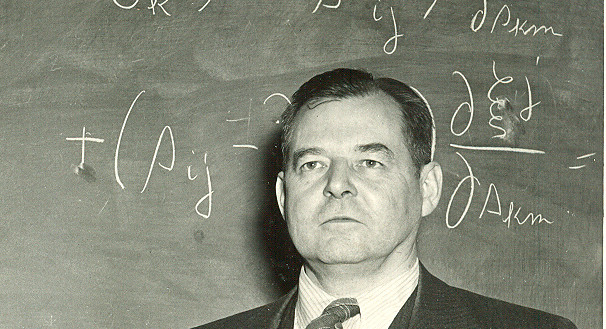
\includegraphics[width=8cm]{./Hotel.jpg}}
\end{picture}

}

\section{Location only}

\frame{\ft{Utility function}
\setbeamertemplate{itemize items}[triangle]

\bi
\item Cost function of consumer: $\tau(|x-l_i|)=t|x-l_i|$
\item Pleasure to consumer: $r$
\item Utility:  $v_i(x)=r-t|x-l_i|$
\item $\overline{p}$
\ei

}

\frame{\ft{Profit function}
\setbeamertemplate{itemize items}[triangle]
$
\pi_i(l_i,l_j) =
\left\{
  \begin{array}{ll}
    (\overline{p}-c )(l_i-l_j )/2 & \mbox{if } l_i < l_j  \\
    (\overline{p}-c)/2 & \mbox{if }  l_i = l_j \\
    (\overline{p}-c )[1-(l_i-l_j )/2] & \mbox{if } l_i > l_j 0 \\
  \end{array}
\right.
$

}

\frame{\ft{General conclusion}
\setbeamertemplate{itemize items}[triangle]



\bi
\item If firms do not choose their prices:  \\
\item They choose not to differentiate \\
\ei

}

\section{Price and location: linear costs}


\frame{\ft{Choosing prices and location}
\setbeamertemplate{itemize items}[triangle]

\bi
\item t = 0: Firms choose where to locate  \\
\item t = 1: Firms choose prices \\
\item t = 2: Consumers go shopping \\
\item Therefore to solve the problem we proceed in this way:\\
\item Step 1: Find the indifferent consumer \\
\item Step 2: Use the indifferent consumer to find the optimal price \\
\item Step 3: Use the optimal price and indifferent consumer to find the location \\
\ei

}



\frame{\ft{Linear costs}
\setbeamertemplate{itemize items}[triangle]

The indifferent consumer is found here:
\begin{align}
r - \tau(\hat{x}-l_1)-p_1  = r - \tau(l_2- \hat{x}) -p_2 \\
\hat{x} = \frac{l_1+l_2}{2}-\frac{p_1-p_2}{2 \tau} \\
\end{align}

We have two conditions for the indifferent consumer to be between the two other firms. 
$
\left\{
  \begin{array}{ll}
    \hat{x} \geq l_1 \leftrightarrow p_1 \leq p_2 + \tau(l_2-l_1)  \\
    \hat{x} \leq l_2 \leftrightarrow p_1 \geq p_2 + \tau(l_2-l_1) \\
  \end{array}
\right.
$

}

\frame{\ft{Indifference point}
\setbeamertemplate{itemize items}[triangle]


\begin{picture}(80,80)(0,0) %syntax: \begin{picture}(width,height)(x-offset,y-offset)
\put(70,-100){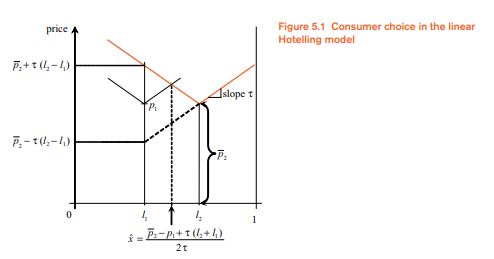
\includegraphics[width=12cm]{./Hotel2.jpg}}
\end{picture}

}

\frame{\ft{Choosing prices and location}
\setbeamertemplate{itemize items}[triangle]
$
\pi_i(p_1,p_2;l_1,l_2) =
\left\{
  \begin{array}{ll}
    0 &\mbox{if } p_1 > p_2 + \tau(l_2-l_1)  \\
    (p_1-c)(\frac{l_1+l_2}{2}+\frac{p_2-p_1}{2})  &\mbox{if } |p_1-p_2| \leq \tau(l_2-l_1)    \\
    (p_1-c) &\mbox{if } p_1 < p_2 - \tau(l_2-l_1)  
  \end{array}
\right.
$

}

\frame{\ft{Indifference point}
\setbeamertemplate{itemize items}[triangle]


\begin{picture}(80,80)(0,0) %syntax: \begin{picture}(width,height)(x-offset,y-offset)
\put(70,-100){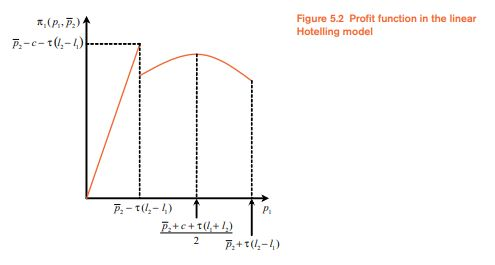
\includegraphics[width=12cm]{./Hotel3.jpg}}
\end{picture}

}

\frame{\ft{Complicated conclusion}
\setbeamertemplate{itemize items}[triangle]


\bi
\item Differentiation does not neccesarily predict a single outcome  \\
\item if firms are far enough apart, there is a unique equilibrium \\
\item But they have a tendency to prefer moving to the center
\ei

}

\section{Price and location: quadratic costs}


\frame{\ft{Quadratic cost}
\setbeamertemplate{itemize items}[triangle]

\begin{align*}
&\text{The cost function} ~~
&& t(|x-l_i|) = \tau (x-l_i)^2 
\\
%%%%%%%%%%%%%%%%%%%%%%%%%%%%%%%%%%%%%%%%%%%%%%%%%
&\text{The indifferent consumer} ~~ 
&& \rightarrow \hat{x}(p_1,p_2) = \frac{l_1+l_2}{2}-\frac{p_1-p_2}{2 \tau (l_1-l_2)}
\\
%%%%%%%%%%%%%%%%%%%%%%%%%%%%%%%%%%%%%%%%%%%%%%%%%
&\text{The profit} ~~ 
&& \pi_1 = (p_2-c)[\hat{x}(p_1,p_2)]
\\
%%%%%%%%%%%%%%%%%%%%%%%%%%%%%%%%%%%%%%%%%%%%%%%%%
&\text{After we take the derivative} ~~
&& p_1^{*} = c+\frac{\tau}{3}(l_2-l_1)(2+l_1+l_2)
\\
%%%%%%%%%%%%%%%%%%%%%%%%%%%%%%%%%%%%%%%%%%%%%%%%%
&\text{And plug it back into } ~~
&& \pi^{*}_1 = \frac{1}{18} \tau (l_2-l_1)(2+l_1+l_2)^2
&\text{If we optimize wrt to the location, we find that $l=0$ } ~~
&& 
\end{align*}


}

\frame{\ft{Conclusion}
\setbeamertemplate{itemize items}[triangle]


\bi
\item Effect 1: Want to be close to center to increase market size  \\
\item Effect 2: Differentiation decreases competition \\
\ei

}
\end{document}